\documentclass{standalone}
\usepackage{tikz}

\usetikzlibrary{calc}

\begin{document}

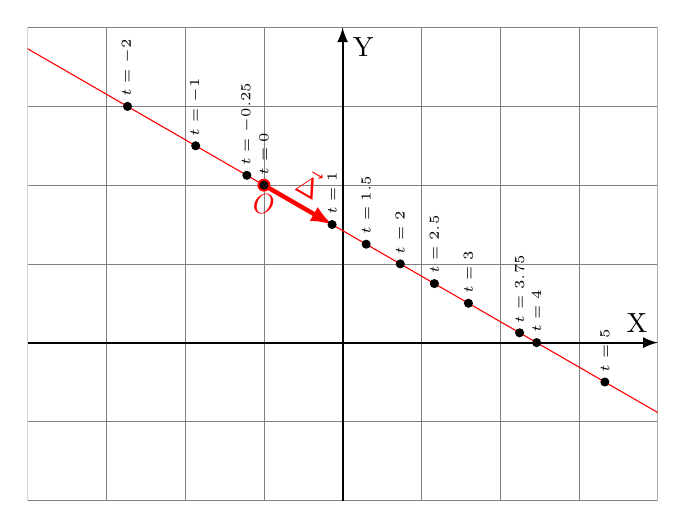
\begin{tikzpicture}[axis/.style={-latex,thick},
                    ray/.style={-latex,ultra thick,red},
                    carrier/.style={red}]
  \path[use as bounding box,clip] (-4,-2) rectangle (4,4);
  \draw[help lines] (-5,-5) grid (5,5);
  \draw[axis] (-4,0) -- (4,0) node[anchor=south east] {X};
  \draw[axis] (0,-4) -- (0,4) node[anchor=north west] {Y};

  \coordinate (origin) at (-1,2);
  \coordinate (through) at ($ (origin) + (-30:1) $);
  \draw[carrier] ($ (origin) ! -10 ! (through) $) -- ($ (origin) ! 10 ! (through) $);
  \draw[ray] (origin) -- (through) node[sloped,above,midway] {$\vec\Delta$};
  \draw[fill=red,red] (origin) circle [radius=0.075cm] node[below] {$O$};

  \foreach \t in {-2,...,5,1.5,2.5,-0.25,3.75} {
    \coordinate (P) at ($ (origin) ! \t ! (through) $);
    \draw[fill=black] (P) circle [radius=0.05cm] node[right,font=\tiny,rotate=90] {$t = \t$};
  }
\end{tikzpicture}

\end{document}